\documentclass[tikz,border=2pt]{standalone}
\usepackage{amsmath,amssymb}
\usepackage{tikz}
\usepackage{pgfplots}
\pgfplotsset{compat=1.18}

\begin{document}
% Phone data K = 605, D = 2, h = 5: setup cost rate KD/y falls, holding rate hy/2 rises, and
% their sum is minimised at y* = sqrt(2KD/h) = 22 where the two are equal (55 + 55 = 110).
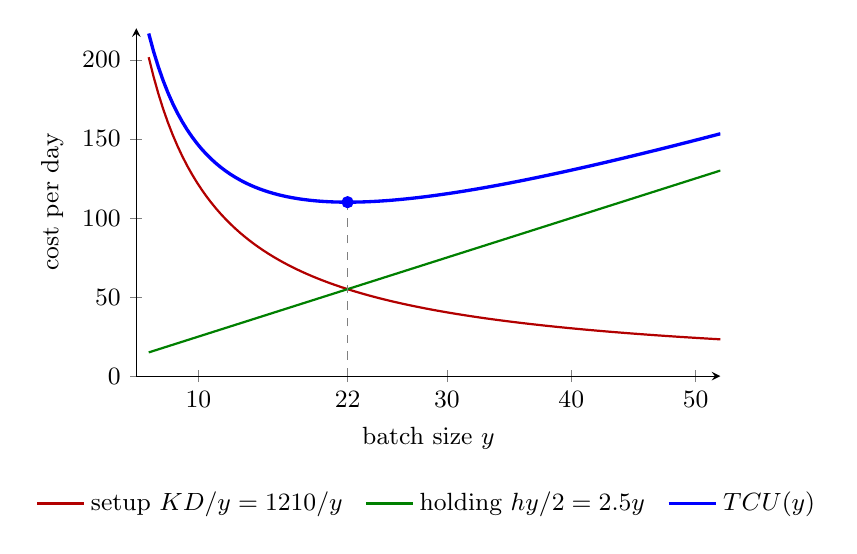
\begin{tikzpicture}
	\begin{axis}[width=9cm, height=6cm, xlabel={batch size $y$}, ylabel={cost per day}, xmin=5, xmax=52, ymin=0, ymax=220, axis lines=left, legend style={at={(0.5,-0.3)}, anchor=north, legend columns=3, font=\small, draw=none, /tikz/every even column/.append style={column sep=6pt}}, tick label style={font=\small}, label style={font=\small}, samples=120, xtick={10,22,30,40,50}]
		\addplot[red!70!black, thick, domain=6:52] {1210/x};
		\addlegendentry{setup $KD/y=1210/y$}
		\addplot[green!50!black, thick, domain=6:52] {2.5*x};
		\addlegendentry{holding $hy/2=2.5y$}
		\addplot[blue, very thick, domain=6:52] {1210/x+2.5*x};
		\addlegendentry{$TCU(y)$}
		\draw[dashed, gray] (axis cs:22,0) -- (axis cs:22,110);
		\addplot[only marks, mark=*, mark size=2pt, blue] coordinates {(22,110)};
	\end{axis}
\end{tikzpicture}
\end{document}
